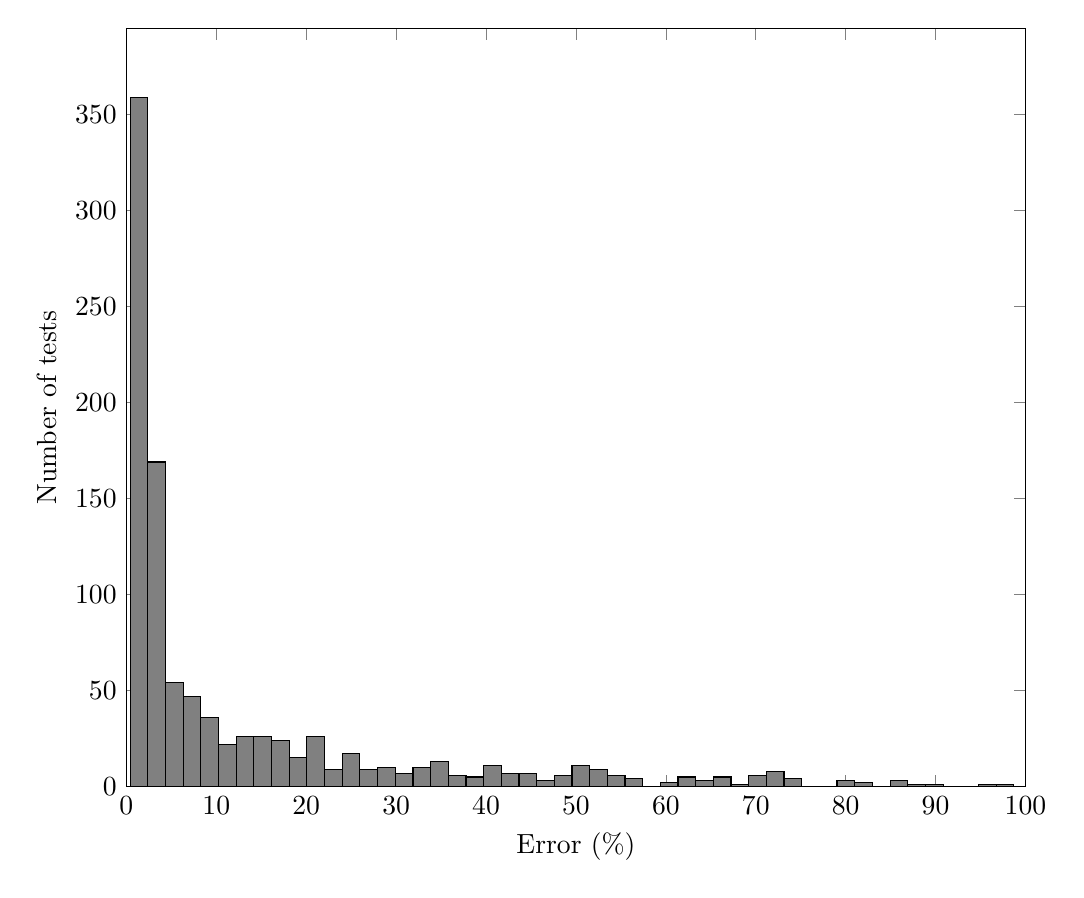
\begin{tikzpicture}
  \begin{axis}[
    width=13cm,
    ylabel=Number of tests,
    xlabel=Error (\%),
    xmin=0,xmax=100,ymin=0,]
    \addplot [ybar interval,fill=gray,draw=black] coordinates {
( 0.42510531, 359.)
( 2.39047363, 169.)
( 4.35584195,  54.)
( 6.32121027,  47.)
( 8.28657859,  36.)
(10.25194691,  22.)
(12.21731523,  26.)
(14.18268355,  26.)
(16.14805187,  24.)
(18.11342019,  15.)
(20.07878851,  26.)
(22.04415683, 9.)
(24.00952515,  17.)
(25.97489347, 9.)
(27.94026179,  10.)
(29.90563011, 7.)
(31.87099843,  10.)
(33.83636675,  13.)
(35.80173507, 6.)
(37.76710339, 5.)
(39.73247171,  11.)
(41.69784003, 7.)
(43.66320835, 7.)
(45.62857667, 3.)
(47.59394499, 6.)
(49.55931331,  11.)
(51.52468163, 9.)
(53.49004995, 6.)
(55.45541827, 4.)
(57.42078659, 0.)
(59.38615491, 2.)
(61.35152323, 5.)
(63.31689155, 3.)
(65.28225987, 5.)
(67.24762819, 1.)
(69.21299651, 6.)
(71.17836483, 8.)
(73.14373315, 4.)
(75.10910147, 0.)
(77.07446979, 0.)
(79.03983811, 3.)
(81.00520643, 2.)
(82.97057475, 0.)
(84.93594307, 3.)
(86.90131139, 1.)
(88.86667971, 1.)
(90.83204803, 0.)
(92.79741635, 0.)
(94.76278467, 1.)
(96.72815299, 1.)
(98.69352131, 0.)
    };
  \end{axis}
\end{tikzpicture}